\chapter{Organización temporal}
\label{chap:org.temporal}

Para la elaboración de este proyecto de fin de carrera me ha sido necesario estudiar de nuevo el funcionamiento de muchos algoritmos sobre grafos que, previamente estudiados durante la titulación, había obviado en ciertos matices que habían que aclara para acometer con precisión una implementación fina y eficiente.\\ Además, la falta de práctica con el lenguaje de programación Java también ha puesto de su parte para la demora de muchos puntos del proyecto.\\

\begin{itemize}
\item Tarea 1:\\

  \begin{enumerate}
  \item Análisis de un software para diagramado de grafos. Descartado por no generar nada más que el fichero gráfico. Se escoge como método de representación en memoria la matriz de adyacencia. Se proyecta el desarrollo de una clase Grafo.java, y adicionalmente otra clase Usa\_Grafo.java que lleven la ejecución principal del programa.
  \item Desarrollo de la clase que dé soporte a los grafos.
    \begin{itemize}
    \item Constructores: nulo y estándar.
    \item Observadores: número de aristas, de nodos, ponderación a nivel de nodos y aristas.
    \item Modificadores: nuevo nodo, nuevas aristas y nueva componente conexa.
    \end{itemize}
  \item Se analiza si los métodos de cálculo sobre grafos formarán de la clase o serán externos.
  \item Comienzo del aprendizaje de NetBeans. Se intenta lograr una primera aproximación a la interfaz de edición de grafos, con generación del soporte en memoria (clase Grafo) por debajo. Que contenga al menos una superficie de dibujo y una botonera para edición/borrado de nodos y aristas. Incluir también un menú básico.
  \end{enumerate}

\item Tarea 2:\\

Desarrollo de la clase que dé soporte a los grafos y sus posteriores métodos.\\

En un primer lugar los métodos de calculo sobre grafos se desarrollarán para la estructura interna del grafo. Aunque no se descarta que posteriormente se cambie dichos métodos a externos. Se podrían colocar externos para facilitar la ocultación de datos para la declaración y definición de tipos grafos, y no tener que preocuparnos de como se accede a los campos internos de la estructura de datos (sea una matriz de adyacencia o de costes). \\

Selecciono una matriz de costes para comprobar los datos internos ya que una matriz de adyacencia podría ser pobre para representar unos valores o duplas tipo vértice y aristas ponderadas asociadas.\\

\item Tarea 3:\\

  Se da formato a la memoria del proyecto con sus partes principales identificables a saber:
  \begin{enumerate}
  \item Previo.
  \item Introducción.
  \item Conceptos básicos.
  \item Algoritmos de Grafos.
  \item Algoritmos Clásicos.
  \item Organización-temporal.
  \item Pruebas.
  \item Conclusiones.
  \item Bibliografía.
  \item GNU Documentation Free License.
  \end{enumerate}

Se continúa desarrollando la codificación para el grafo en el fichero Grafo.java. Primeros problemas con la forma de trabajar con la matriz interna ya que supondría un coste muy elevado el estar constantemente haciendo 2 bucles para inserción y/o eliminación y búsqueda de vértices/nodos y de aristas.\\

\item Tarea 4:\\
Codificación final del fichero Grafo.java. Comenzando edición del fichero Usa\_grafo que implementará objetos del tipo Grafo y que servirá para una primera toma de contacto con la estructura de datos del grafo y sus métodos implementados.\\

Se consigue una propuesta en lenguaje de programación para la comprobación de si un grafo es conexo o no. \\

\item Tarea 5:\\
Compilación de los ficheros Grafo.java y Usa\_grafo.java y depuración de errores encontrados, restituyendo variables erróneas o añadiendo métodos correctos para las clases contenedoras y tipos primitivos.\\

Dudas con respecto a la posible asignación o creación de un ArrayList de tipo boolean y de un Set de tipo int (entero).\\

\item Tarea 6:\\
He tenido problemas con el redimensionamiento de los Arraylist en memoria ya que cuando asignaba los vértices con sus correspondientes aristas me almacenaba para un vértice de mas que no utilizaba y por ello tuve que realizar nuevas modificaciones en el código fuente desarrollado hasta la fecha en Grafo.java y Usa\_grafo.java. He solucionado el problema modificando, en el método nueva\_arista, el método para el ArrayList add por set que establece el elemento en la posición especificada y si hay otro elemento lo re-escribe en la misma posición de memoria.

\begin{Verbatim}[commandchars=\\\{\}]
\PY{n}{rep\PYZus{}grafo}\PY{o}{.}\PY{n+na}{get}\PY{o}{(}\PY{n}{vertice\PYZus{}i}\PY{o}{)}\PY{o}{.}\PY{n+na}{add}\PY{o}{(}\PY{n}{vertice\PYZus{}j}\PY{o}{,}\PY{n}{peso}\PY{o}{)}\PY{o}{;}
\end{Verbatim}


por

\begin{Verbatim}[commandchars=\\\{\}]
\PY{n}{rep\PYZus{}grafo}\PY{o}{.}\PY{n+na}{get}\PY{o}{(}\PY{n}{vertice\PYZus{}i}\PY{o}{)}\PY{o}{.}\PY{n+na}{set}\PY{o}{(}\PY{n}{vertice\PYZus{}j}\PY{o}{,}\PY{n}{peso}\PY{o}{)}\PY{o}{;}
\end{Verbatim}


Quedando así solucionado el problema, además de que así puede insertar las aristas siguiendo la numeración o etiquetado de los nodos o vértices del nodo, es decir, [vertice\_i,vertice\_j] = peso. p.ejemplo: [0,1] = 4. Siendo 0 incidente sobre 1.\\

También se consigue solucionar el problema de la creación de un ArrayList de boolean y de un Set de int. Consistía en declarar su tipo como Boolean e Integer respectivamente. No sé el porqué de dicho problema pero esta relacionado con la clase Integer y supongo que con la clase Boolean.\\

Se comentan los nuevo métodos explicando los parámetros formales, los tipos de retorno en el caso que haya y la funcionalidad del método.\\

\item Tarea 7:\\
\begin{enumerate}
\item La clase Grafo ha sido diseñada a nivel de métodos o constructores y de métodos básicos. Hay problemas con determinados métodos. Se ha tenido en cuenta el paso a una matriz de adyacencia desde una representación basa en HashMap.. El diseño actual supone de forma obligatoria que existe una función de coste asociada a las aristas. Esto es demasiado restrictivo y no permite computar sobre grafos sin función de coste.
\item Se dispone de un método aritmético para verificar la conexión de un determinado grafo. Es necesario verificar que ese resultado es matemáticamente consistente.
\item Con el método de adición de nuevas componente, hay dificultades. Se sugiere utilizar como representación intermedia la matricial para facilitar la operación.-
\item Se decide incorporar los métodos de cálculo fuera de la clase que implementa al grafo.
\end{enumerate}

Nuevas líneas de trabajo a desarrollar:
\begin{itemize}
\item Comenzar a implantar algoritmos de computación sobre grafos.
\item Comenzar a aprender NetBeans.
\end{itemize}

Hay un método llamada Arrays.deepToString("colocamos la variable matriz") que transforma a tipo String cualquier tipo de array multidimensional, sea de la dimensión que sea, pero el formato no es el deseado. Aún así no se descarta su utilización para posteriores comprobaciones de una matriz o devolución por salida estándar.\\

He descubierto un nuevo método de la clase Collections, en concreto, Collections.nCopies(). El cual para un tamaño del tipo (en este caso un tamaño ArrayList.size()) y para un elemento del tipo que sea (para definir el ArrayList lo hago al valor nulo 0) copia dicho elemento en todas las posiciones del ArrayList o Collections que se trate.\\
nCopies(int n, T o): Returns an immutable list consisting of n copies of the specified object.\\

Cambiamos la implementación del método es\_conexo por la fórmula matemática que comprueba si es o no conexa una componente a través de sus aristas (cardinal) y sus vértices (cardinal).\\

Siguen existiendo problemas con el método nueva\_componente ya que hay que redimensionar el tamaño de las columnas para toda la estructura anterior y añadir los nuevos nodos y aristas de la nueva componente. Se emplea la conversión a tipo Array multidimensional para facilitar la vida al programador.\\

Vuelve a ocurrir lo de la memoria dinámica con java. Tengo que re-definir la variable matriz\_devuelta para que los valores del ArrayList se actualicen en la nueva pasada.\\

\begin{Verbatim}[commandchars=\\\{\}]
\PY{n}{ArrayList}\PY{o}{<}\PY{n}{Integer}\PY{o}{>} \PY{n}{matriz\PYZus{}devuelta} 
    \PY{o}{=} \PY{k}{new} \PY{n}{ArrayList}\PY{o}{<}\PY{n}{Integer}\PY{o}{>}\PY{o}{(}\PY{n}{Collections}\PY{o}{.}\PY{n+na}{nCopies}\PY{o}{(}\PY{n}{tama\PYZus{}g}\PY{o}{+}\PY{n}{ultimo\PYZus{}indice}\PY{o}{,}\PY{l+m+mi}{0}\PY{o}{)}\PY{o}{)}\PY{o}{;}
\end{Verbatim}


Uso la variable ultimo\_indice para insertar las posiciones de las nuevas aristas de la componente en la estructura principal. Para ello hemos de saber que la dimensión de la estructura principal es desde 0-size() (rep\_grafo) y que para la nueva componente será de size()-size()+n siendo n el número de nodos que tenga la nueva componente. El valor de size() original se guarda en ultimo\_indice para evitar que se modifique cuando se amplíe la dimensión de la estructura.\\

Se consigue que todos los métodos realizados hasta la fecha compilen y ejecuten sin ningún tipo de error. Faltar por añadir la sobrecarga de la clase Grafo para Grafos no ponderados y falta añadir una nueva clase Envoltorio que cree la independencia del TAD sobre su implementación. Principio fundamental de la ocultación de datos y forma de facilitar la vida al programador.\\

\item Tarea 8:\\
Añado una nueva clase llamada Envoltorio que contendrá la estructura interna de la representación del grafo. Redefinimos la codificación de Grafo.java para adaptarla a la nueva clase y añadimos un nuevo método privado llamado "private Envoltorio devolver\_estruc\_interna()".\\

Dicho método devolverá la estructura interna que emplea la clase Grafo para trabajar con los objetos de Envoltorio, en este caso para el atributo privado declarado dentro de la clase Grafo. Con el principio de ocultación private el método solo será accesible desde dentro de la clase, o sólo podrá invocarse el método desde otro método de la clase.\\

Se compilan y ejecutan todos los fichero con la nueva codificación y no hay ningún problema.\\

Se define una primera aproximación del algoritmo de Dijkstra en java. Para poder mostrar en un momento posterior al computo del algoritmo se emplea una estructura de datos en formato array multidimensional en donde la fila 0 se hayan los costes asociados al cálculo de Dijkstra y en la fila 1 se encuentran los caminos mínimos, desde un origen, obtenidos en la computación anterior.\\

Se haya un problema con el algoritmo de Floyd, ya que si queremos mostrar el camino recorrido por el algoritmo para sus distintos vértices tenemos que realizar dicha traza al finalizar el algoritmo justo antes de la devolución del tipo especifico de la función.\\

\item Tarea 9:\\
Añadiendo más funcionales a los métodos de la clase Algoritmos. Se añade los siguientes métodos:

\begin{Verbatim}[commandchars=\\\{\}]
\PY{k+kd}{public} \PY{k+kt}{int}\PY{o}{[}\PY{o}{]} \PY{n+nf}{recorrido\PYZus{}profundidad}\PY{o}{(}\PY{o}{)}
\PY{k+kd}{public} \PY{k+kt}{int}\PY{o}{[}\PY{o}{]} \PY{n+nf}{recorrido\PYZus{}anchura}\PY{o}{(}\PY{o}{)}
\PY{k+kd}{public} \PY{k+kt}{boolean} \PY{n+nf}{AciclicoGD}\PY{o}{(}\PY{k+kt}{int} \PY{o}{[}\PY{o}{]}\PY{o}{[}\PY{o}{]} \PY{n}{G}\PY{o}{)}
\PY{k+kd}{static} \PY{k+kt}{boolean} \PY{n+nf}{AciclicoGDRec}\PY{o}{(}\PY{k+kt}{int} \PY{n}{vertice}\PY{o}{,} \PY{k+kt}{int} \PY{o}{[}\PY{o}{]}\PY{o}{[}\PY{o}{]} \PY{n}{G}\PY{o}{,} \PY{k+kt}{int} \PY{n}{num\PYZus{}ancestros}\PY{o}{)}
\PY{k+kd}{private} \PY{k+kt}{boolean} \PY{n+nf}{AciclicoGND}\PY{o}{(}\PY{o}{)} 
\PY{k+kd}{static} \PY{k+kt}{boolean} \PY{n+nf}{AciclicoGNDRec}\PY{o}{(}\PY{o}{)}
\end{Verbatim}


He encontrado un problema muy importante en java que no sabía y es que no tiene paso por referencia entre funciones o cualquier tipo de operación sobre la que trabajemos, además de que no se pueden especificar tipos específicos para cualquier tipo de variable. Los nuevos tipos se han de definir como clases enteras para poder trabajar con ellas. El problema del paso por copia de todos los objetos conlleva que para simular dicho paso por referencia hay que declarar esa variable como un atributo privado de la clase en el método (privado) que solo será accesible por un objeto de esa clase y sólo de esa clase. No se podrá exportar fuera de ella a no ser que sea a través de un método observador que nos permita trabajar con él o con algún dato asociado.\\

\item Tarea 10:\\
Si empleamos los métodos o algoritmos de acíclico hemos de tener en cuenta una cosa; solo podemos usar uno de los 2 una sola vez por cada uno de ellos ya que cada método principal inicializa el atributo privado de la clase cada vez para su propio método recursivo.\\

Se termina de definir los métodos o funciones para comprobar si el grafo de entrada tiene ciclos en su estructura o no. Se comentan los prototipos de las funciones disponibles hasta el momento para la clase Algoritmos.\\

Al compilar el fichero me dice que para los prototipos declarados como static no se puede acceder a atributos privados de la clase contenedora, por lo que he tenido de declarar dichos métodos como private.\\

Al compilar el fichero se depuran algunos errores y se prosigue.\\

Para el método de recorrido en profundidad sucede lo mismo que para otros algoritmos ya que hay que pasar un vector o variable por referencia y como se permite tendremos que crear un nuevo atributo privado de la clase que sólo sea accesible desde dentro de ella y para el método en concreto que sea necesario.\\

He descubierto que para emplear la estructura de datos cola tengo que emplear la clase LinkedList. Una cola es un contenedor "first-in, first-out" FIFO (el primero en entrar es el primero en salir). Es decir, se introducen los elementos por un extremo y se sacan por el otro. Por tanto, los elementos se extraerán en el mismo orden en que fueron introducidos. LinkedList tiene métodos para soportar el comportamiento de una cola, que pueden usarse en una clase Cola.\\

He implementado el método recorrido\_anchura empleando la clase LinkedList que implementa una cola. Dicha cola nos servirá para ir almacenando, en un orden correcto, los vértices visitados para ir procesándolos según sea.\\

IMPORTANTE: Hay que hacer algo para que los costes de los algoritmos sean en valor absoluto ya que para valores negativos debería ser ya que provocaría un error al encontrar el menor valor posible de todos los del rango positivo, vamos que el negativo sería con diferencia el menor de todos.\\

\item Tarea 11:\\
Se buscan posibles soluciones para la implementación del algoritmo de Kruskal sin emplear una partición de conjuntos del grafo. Pero todos las referencias indican que esa representación es la más adecuada para trabajar con las componentes del grafo. Además se encuentra el problema de que hay demasiado tipos que deben definirse como clases o estructuras nuevas independientes de los tipos primitivos del lenguaje java en este caso.\\

\item Tarea 12:\\
Se decide implementar la clase partición después de hacer una traza sobre un ejemplo aleatorio y realizar un adaptación al lenguaje de programación.\\

Se implementa la clase Arista que contendrá los atributos privados; origen, destino y coste para cada par de arista correspondiente. Se implementa el método interno de la clase Algoritmo QuickSort que será dicho conocido algoritmo adaptado al lenguaje java. Se define un nuevo atributo privado de la clase Algoritmo que se llamará Arist y será un ArrayList de elementos <Arista>.\\

Cambiando tipo de acceso del método Quicksort de static a private.\\

Se han compilado todos los ficheros existentes ``.java'' (Grafo,Usa\_grafo,Algoritmos,\\Envoltorio,Partición,Arista). 
Se depuran fallos en tiempo de compilación.\\

Como tenemos una nueva clase llamada Arista, podemos cambiar la forma de trabajo con los algoritmos. Usaremos ArrayList cuya eficiencia puede resultar mejor que para arrays de 2 dimensiones, además de las operaciones que nos aporta este tipo de contenedor respecto a un array simple.\\

Hacemos cambios en el método algo\_Prim que tendrá como parámetro de devolución un ArrayList<Arista> en sustitución de la técnica anterior que simulaba una arista con dos filas de una matriz.

\begin{Verbatim}[commandchars=\\\{\}]
\PY{c+cm}{/**}
\PY{c+cm}{ * Método observador (Algoritmo de Prim)}
\PY{c+cm}{ * Devuelve en un vector el conjunto de aristas que forman un árbol}
\PY{c+cm}{ * generador de coste mínimo de un grafo conexo.}
\PY{c+cm}{ * @param G matriz de costes asociada al grafo G}
\PY{c+cm}{ * @return una matriz booleana de tamaño 2xN que sera el conjunto de }
\PY{c+cm}{ * aristas que forman un árbol generador de coste mínimo del grafo }
\PY{c+cm}{ * de entrada (matriz). La fila 0 tendra el vértice origen y la }
\PY{c+cm}{ * fila 1 correlativa contendrá el vértice destino (formando así }
\PY{c+cm}{ * pares de elementos)}
\PY{c+cm}{ * @exception Exception}
\PY{c+cm}{ */}
\end{Verbatim}


A esto

\begin{Verbatim}[commandchars=\\\{\}]
\PY{c+cm}{/**}
\PY{c+cm}{ * Método observador (Algoritmo de Prim)}
\PY{c+cm}{ * Devuelve en un vector el conjunto de aristas que forman un árbol}
\PY{c+cm}{ * generador de coste minimo de un grafo conexo.}
\PY{c+cm}{ * @param G matriz de costes asociada al grafo G}
\PY{c+cm}{ * @return devuelve un ArrayList con el conjunto de aristas que }
\PY{c+cm}{ * forman un árbol generador de coste mínimo del grafo conexo G.}
\PY{c+cm}{ * @exception Exception}
\PY{c+cm}{ */}
\end{Verbatim}


Se compilan los nuevos cambios. No se produce ningún error.\\

Se documentan las clases o ficheros nuevos (Partición,Arista,Envoltorio,Algoritmos) para los métodos que sean necesarios.\\

Primera prueba sobre los algoritmo empleando la clase Grafo.\\

\item Tarea 13:\\
Se crear nuevos métodos en la clase Grafo para el uso de los algoritmos de la clase Algoritmos.\\

Hay que modificar la estructura de los métodos de la clase Envoltorio para que asigne valores mayores que cero (infinito) en las matrices de costes para que se pueda operar con los algoritmos sobre grafos. Para ello se añade en los constructores la línea "Collections.fill(lista,100)" siendo 100 el valor infinito o de mayor coste posible.\\

También hay que modificar los métodos de inserción de nuevo nodo o nueva componente para que realice la misma operación.\\

Método \_nodo\_nuevo\_ añado 100 en esta línea.\\

\begin{Verbatim}[commandchars=\\\{\}]
\PY{n}{rep\PYZus{}grafo}\PY{o}{.}\PY{n+na}{get}\PY{o}{(}\PY{n}{o}\PY{o}{)}\PY{o}{.}\PY{n+na}{add}\PY{o}{(}\PY{n}{vertices\PYZus{}grafo}\PY{o}{.}\PY{n+na}{size}\PY{o}{(}\PY{o}{)}\PY{o}{-}\PY{l+m+mi}{1}\PY{o}{,}\PY{l+m+mi}{100}\PY{o}{)}\PY{o}{;}
\PY{n}{Collections}\PY{o}{.}\PY{n+na}{fill}\PY{o}{(}\PY{n}{vertices\PYZus{}grafo}\PY{o}{,}\PY{l+m+mi}{100}\PY{o}{)}\PY{o}{;}
\end{Verbatim}


Método \_componente\_nueva\_ añado 100 en esta línea.\\

\begin{Verbatim}[commandchars=\\\{\}]
\PY{n}{rep\PYZus{}grafo}\PY{o}{.}\PY{n+na}{get}\PY{o}{(}\PY{n}{o}\PY{o}{)}\PY{o}{.}\PY{n+na}{add}\PY{o}{(}\PY{n}{ultimo\PYZus{}indice}\PY{o}{+}\PY{n}{i}\PY{o}{,}\PY{l+m+mi}{100}\PY{o}{)}\PY{o}{;}
\PY{n}{ArrayList}\PY{o}{<}\PY{n}{Integer}\PY{o}{>} \PY{n}{matriz\PYZus{}devuelta}\PY{o}{.}\PY{o}{.}\PY{o}{.}\PY{o}{.}\PY{o}{.}\PY{o}{.}\PY{o}{(}\PY{n}{tama\PYZus{}g}\PY{o}{+}\PY{n}{ultimo\PYZus{}indice}\PY{o}{,}\PY{l+m+mi}{100}\PY{o}{)}\PY{o}{;}
\end{Verbatim}


Se modifican correctamente las estructura internas con ese nuevo valor máximo.\\

Método Envoltorio(int n).\\

\begin{Verbatim}[commandchars=\\\{\}]
\PY{n}{Collections}\PY{o}{.}\PY{n+na}{fill}\PY{o}{(}\PY{n}{lista}\PY{o}{,}\PY{l+m+mi}{100}\PY{o}{)}\PY{o}{;}
\PY{n}{vertices\PYZus{}grafo}\PY{o}{.}\PY{n+na}{add}\PY{o}{(}\PY{l+m+mi}{100}\PY{o}{)}\PY{o}{;}
\end{Verbatim}


El problema que había es que para el algoritmo de Dijkstra, al pasar la matriz de costes del grafo a la matriz de costes interna se iteraba sobre n-1 y no sobre n quedando la posición (v==3) con el valor 0 haciendo que el resultado no fuera válido. Se soluciona el problema. \\

\begin{Verbatim}[commandchars=\\\{\}]
\PY{k}{for}\PY{o}{(}\PY{n}{v}\PY{o}{=}\PY{l+m+mi}{0}\PY{o}{;} \PY{n}{v} \PY{o}{<} \PY{n}{tama\PYZus{}G}\PY{o}{;} \PY{o}{+}\PY{o}{+}\PY{n}{v}\PY{o}{)}
    \PY{o}{\PYZob{}}
	\PY{n}{Costes\PYZus{}Vertices}\PY{o}{[}\PY{l+m+mi}{0}\PY{o}{]}\PY{o}{[}\PY{n}{v}\PY{o}{]} \PY{o}{=} \PY{n}{G}\PY{o}{[}\PY{n}{origen}\PY{o}{]}\PY{o}{[}\PY{n}{v}\PY{o}{]}\PY{o}{;}

	\PY{c+c1}{//Asignamos todos los costes asociados partiendo desde}
	\PY{c+c1}{//el vertice origen}
	\PY{n}{Costes\PYZus{}Vertices}\PY{o}{[}\PY{l+m+mi}{1}\PY{o}{]}\PY{o}{[}\PY{n}{v}\PY{o}{]} \PY{o}{=} \PY{n}{origen}\PY{o}{;}
	\PY{c+c1}{//El vector tiene como elementos al vertice origen}
    \PY{o}{\PYZcb{}}
\end{Verbatim}


en vez de\\

\begin{Verbatim}[commandchars=\\\{\}]
\PY{k}{for}\PY{o}{(}\PY{n}{v}\PY{o}{=}\PY{l+m+mi}{0}\PY{o}{;} \PY{n}{v} \PY{o}{<} \PY{n}{tama\PYZus{}G}\PY{o}{-}\PY{l+m+mi}{1}\PY{o}{;} \PY{o}{+}\PY{o}{+}\PY{n}{v}\PY{o}{)}
    \PY{o}{.}\PY{o}{.}\PY{o}{.}\PY{o}{.}
\end{Verbatim}


Modifico el método\_aristas\_numero() de la clase Envoltorio en la línea\\

\begin{Verbatim}[commandchars=\\\{\}]
 \PY{k}{if}\PY{o}{(}\PY{n}{rep\PYZus{}grafo}\PY{o}{.}\PY{n+na}{get}\PY{o}{(}\PY{n}{o}\PY{o}{)}\PY{o}{.}\PY{n+na}{get}\PY{o}{(}\PY{n}{i}\PY{o}{)} \PY{o}{>} \PY{l+m+mi}{0} \PY{o}{&}\PY{o}{&} \PY{n}{o} \PY{o}{!}\PY{o}{=} \PY{n}{i}\PY{o}{)}	
\end{Verbatim}


a \\

\begin{Verbatim}[commandchars=\\\{\}]
 \PY{k}{if}\PY{o}{(}\PY{n}{rep\PYZus{}grafo}\PY{o}{.}\PY{n+na}{get}\PY{o}{(}\PY{n}{o}\PY{o}{)}\PY{o}{.}\PY{n+na}{get}\PY{o}{(}\PY{n}{i}\PY{o}{)} \PY{o}{>} \PY{l+m+mi}{0} 
    \PY{o}{&}\PY{o}{&} \PY{n}{o} \PY{o}{!}\PY{o}{=} \PY{n}{i} \PY{o}{&}\PY{o}{&} \PY{n}{rep\PYZus{}grafo}\PY{o}{.}\PY{n+na}{get}\PY{o}{(}\PY{n}{o}\PY{o}{)}\PY{o}{.}\PY{n+na}{get}\PY{o}{(}\PY{n}{i}\PY{o}{)} \PY{o}{<} \PY{l+m+mi}{100}\PY{o}{)}
\end{Verbatim}


Dado que ahora existe una cifra máximo para los costes y si el valor esta comprendido entres esos valores es que existe arista.\\

Redefino el método Algoritmo de Warshall para trabajar con una matriz de enteros en vez de una matriz booleana, ya que con enteros es más fácil su representación en el flujo de salida estándar.\\

Me defino un método privado nuevo para la clase Grafo llamado void mostrar\_matriz\_pantalla(), que servirá para mostrar por el flujo de salida el contenido del grafo en formato matriz.\\

Hay otro problema al definir los métodos de inserción de nodo y componente con un valor infinito, véase 100. Para una matriz de adyacencia no es posible este procedimiento, por lo que se modifica nuevamente la cabecera y la estructura interna de los métodos:\\

\begin{Verbatim}[commandchars=\\\{\}]
\PY{k+kd}{public} \PY{k+kt}{void} \PY{n+nf}{\PYZus{}nodo\PYZus{}nuevo\PYZus{}}\PY{o}{(}\PY{k+kt}{int} \PY{n}{x}\PY{o}{,} \PY{k+kt}{int} \PY{n}{y}\PY{o}{)}\PY{o}{;}

\PY{k+kd}{public} \PY{k+kt}{void} \PY{n+nf}{\PYZus{}componente\PYZus{}nueva\PYZus{}}\PY{o}{(}\PY{n}{Envoltorio} \PY{n}{g}\PY{o}{)}\PY{o}{;}
\end{Verbatim}


a\\

\begin{Verbatim}[commandchars=\\\{\}]
\PY{k+kd}{public} \PY{k+kt}{void} \PY{n+nf}{\PYZus{}nodo\PYZus{}nuevo\PYZus{}}\PY{o}{(}\PY{k+kt}{int} \PY{n}{x}\PY{o}{,} \PY{k+kt}{int} \PY{n}{y}\PY{o}{,} \PY{k+kt}{int} \PY{n}{infinito}\PY{o}{)}\PY{o}{;}

\PY{k+kd}{public} \PY{k+kt}{void} \PY{n+nf}{\PYZus{}componente\PYZus{}nueva\PYZus{}}\PY{o}{(}\PY{n}{Envoltorio} \PY{n}{g}\PY{o}{,} \PY{k+kt}{int} \PY{n}{infinito}\PY{o}{)}\PY{o}{;}
\end{Verbatim}


infinito: valor entero que especifica si el contenido de la matriz es para una matriz de adyacencia o de costes (adyacente->infinito==0, !adyacente->infinito==100).\\

Hemos de añadir también una variable o algún mecanismo de control para saber si el grafo es dirigido o no dirigido. Para ello modifico la cabecera de los constructores del Grafo y añado sentencias condicionadas por ello en las inserciones de arista para que se añadan en ambas direcciones o no.\\

También hay que modificar la cabecera del método \_arista\_nueva\_ de la clase Envoltorio por lo sucedido en la anterior línea.\\

\begin{Verbatim}[commandchars=\\\{\}]
\PY{k+kd}{public} \PY{k+kt}{void} \PY{n+nf}{\PYZus{}arista\PYZus{}nueva\PYZus{}} \PY{o}{(}\PY{k+kt}{int} \PY{n}{v\PYZus{}i}\PY{o}{,} \PY{k+kt}{int} \PY{n}{v\PYZus{}j}\PY{o}{,} \PY{k+kt}{int} \PY{n}{x}\PY{o}{,} \PY{k+kt}{boolean} \PY{n}{diri}\PY{o}{)}
\PY{o}{\PYZob{}}

    \PY{k}{if}\PY{o}{(}\PY{n}{v\PYZus{}i} \PY{o}{<} \PY{n}{num\PYZus{}nodos\PYZus{}} \PY{o}{|}\PY{o}{|} \PY{n}{v\PYZus{}j} \PY{o}{<} \PY{n}{num\PYZus{}nodos\PYZus{}}\PY{o}{)}
	\PY{o}{\PYZob{}}
	    \PY{k}{if}\PY{o}{(}\PY{n}{v\PYZus{}i} \PY{o}{!}\PY{o}{=} \PY{n}{v\PYZus{}j}\PY{o}{)}
		\PY{o}{\PYZob{}}
		    \PY{n}{rep\PYZus{}grafo}\PY{o}{.}\PY{n+na}{get}\PY{o}{(}\PY{n}{v\PYZus{}i}\PY{o}{)}\PY{o}{.}\PY{n+na}{set}\PY{o}{(}\PY{n}{v\PYZus{}j}\PY{o}{,}\PY{n}{x}\PY{o}{)}\PY{o}{;}
		    \PY{k}{if}\PY{o}{(}\PY{n}{diri}\PY{o}{)}
			\PY{n}{rep\PYZus{}grafo}\PY{o}{.}\PY{n+na}{get}\PY{o}{(}\PY{n}{v\PYZus{}j}\PY{o}{)}\PY{o}{.}\PY{n+na}{set}\PY{o}{(}\PY{n}{v\PYZus{}i}\PY{o}{,}\PY{n}{x}\PY{o}{)}\PY{o}{;}
			
		\PY{o}{\PYZcb{}}
	    \PY{k}{else}
		\PY{o}{\PYZob{}}
		    \PY{k}{if}\PY{o}{(}\PY{n}{adyacente}\PY{o}{)}
			\PY{o}{\PYZob{}}
			    \PY{n}{rep\PYZus{}grafo}\PY{o}{.}\PY{n+na}{get}\PY{o}{(}\PY{n}{v\PYZus{}i}\PY{o}{)}\PY{o}{.}\PY{n+na}{set}\PY{o}{(}\PY{n}{v\PYZus{}j}\PY{o}{,}\PY{l+m+mi}{1}\PY{o}{)}\PY{o}{;}
			    \PY{k}{if}\PY{o}{(}\PY{n}{diri}\PY{o}{)}
				\PY{n}{rep\PYZus{}grafo}\PY{o}{.}\PY{n+na}{get}\PY{o}{(}\PY{n}{v\PYZus{}j}\PY{o}{)}\PY{o}{.}\PY{n+na}{set}\PY{o}{(}\PY{n}{v\PYZus{}i}\PY{o}{,}\PY{l+m+mi}{1}\PY{o}{)}\PY{o}{;}
			\PY{o}{\PYZcb{}}
		\PY{o}{\PYZcb{}}
		    
	\PY{o}{\PYZcb{}}
    \PY{k}{else}
	\PY{n}{System}\PY{o}{.}\PY{n+na}{out}\PY{o}{.}\PY{n+na}{println}\PY{o}{(}\PY{l+s}{"No existe el nodo: Lanzar exepcion"}\PY{o}{)}\PY{o}{;}
       
\PY{o}{\PYZcb{}}
\end{Verbatim}


Hay un problema con el algoritmo de Prim ya que procesa adecuadamente los nodos y sus respectivos conjuntos de aristas, pero a la hora de almacenarlos en el ArrayList no lo hace correctamente y machaca el último conjunto de nodos posibles.
Solución a este problema: muy simple, java y su genial controlador de memoria dinámica reasignaba el valor una y otra vez al ArrayList por cada modificación del (Arista) ``a'' anterior en la sentencia condicional if(G[j][k] <= CosteMin). Con lo que en cada llamada a esta sentencia se tiene que crear un nuevo objeto de la clase Arista, sea ``a'', y volver a almacenar los nuevos datos.\\

\item Tarea 14:\\
Se intenta hacer funcionar el algoritmo de Kruskal sin éxito. \\
Misteriosamente no puedo añadir una nueva componente de tipo adyacente a un grafo anterior del mismo tipo.\\
Hay que documentar los nuevo métodos creados.\\
Se obtiene un ejemplo para todos los tipos de métodos posibles. \\
Funcionan correctamente:
\begin{itemize}
\item Floyd
\item Dijkstra
\item Prim
\item Conexo
\item Aciclico
\item rec\_anchura
\item rec\_profundidad
\end{itemize}

\item Tarea 15:\\

Añadir más algoritmos a la estructura de datos:\\

\begin{itemize}
\item Ciclo Hamiltoniano.
\item Comprobar si un grafo es completo o no.
\item Teorema de los 4 colores.
\item Coloreado de grafos.
\item Comprobar si un grafo es plano o no.
\item Intentar orden topológico.
\item Intentar teorema de Kuratowski.
\item Representar el problema de los puentes de Königsberg.
\end{itemize}

Empleo el método clone de la clase ArrayList para clonar o copiar un contenido en otro ArrayList; La verdad no resulta muy útil para mi problema y se descarta de momento.\\

Soluciono el error de comprobación de si un grafo es dirigido o no ya que el valor del condicional estaba colocado en orden inverso al que se pretendía,es decir, había que poner if(!dirigido) para que funcione correctamente.\\

Volvemos a verificar que funciona los grafos dirigidos y no dirigidos para la creación.\\

Parece que la función nuevo nodo no funciona adecuadamente. Y el motivo era que en rep\_grafo.get(o)..... estaba con el índice puesto en vertices\_size() que era incorrecto, había que poner rep\_grafo.get(o).add(aux,infinito);\\

\begin{Verbatim}[commandchars=\\\{\}]
\PY{k}{for}\PY{o}{(}\PY{k+kt}{int} \PY{n}{aux}\PY{o}{=}\PY{l+m+mi}{0}\PY{o}{;} \PY{n}{aux} \PY{o}{<} \PY{n}{rep\PYZus{}grafo}\PY{o}{.}\PY{n+na}{size}\PY{o}{(}\PY{o}{)}\PY{o}{-}\PY{l+m+mi}{1} \PY{o}{&}\PY{o}{&} \PY{n}{it}\PY{o}{.}\PY{n+na}{hasNext}\PY{o}{(}\PY{o}{)}\PY{o}{;} \PY{o}{+}\PY{o}{+}\PY{n}{aux}\PY{o}{)}
    \PY{o}{\PYZob{}}
	\PY{n}{Object} \PY{n}{o} \PY{o}{=} \PY{n}{it}\PY{o}{.}\PY{n+na}{next}\PY{o}{(}\PY{o}{)}\PY{o}{;}
	\PY{n}{rep\PYZus{}grafo}\PY{o}{.}\PY{n+na}{get}\PY{o}{(}\PY{n}{o}\PY{o}{)}\PY{o}{.}\PY{n+na}{add}\PY{o}{(}\PY{n}{aux}\PY{o}{,}\PY{n}{infinito}\PY{o}{)}\PY{o}{;}
    \PY{o}{\PYZcb{}}
\end{Verbatim}


Misteriosamente nueva\_componente hace lo que hace nuevo\_nodo y mejor..en fin. Tendré que modificar de nuevo nuevo\_nodo desde la clase Envoltorio.\\

\item Tarea 16:\\

Intento cambiar la definición del método de la clase Envoltorio \_nodo\_nuevo\_ porque parece que no realiza la inserción correctamente.\\

He sobrecargado la función nuevo\_nodo en la clase Grafo para que no tengamos que pasar obligatoriamente un peso para el nodo, pero si obligatoriamente su componente a la que pertenece.\\

El error que daba en devolver matriz supuestamente era porque reservaba para el tamaño de vertices\_grafo que era menor que el de rep\_grafo. solución: doy el tamaño de rep\_grafo para la matriz. Pero ahora asigno las nuevas columnas a la matriz con ceros en vez de con infinitos.\\

Solucionado el problema de que cuando añadimos un nuevo nodo el índice sea mayor que el tamaño de la estructura a la que se accede. Solución: int tama\_g = rep\_grafo.size()+1; en el método \_nodo\_nuevo(int x, int y, int componente). El tema esta en el +1 ese para que tenga un elemento de más que en c podría ser como el caracter de fin de cadena. \\

Ahora parece que va todo bien, como la seda (pero no he probado los algoritmos sobre las estructuras).\\

Añado un nuevo método a la clase Grafo(privado) es\_adyacencia para comprobar si la matriz del grafo es de adyacencia o no y así poder trabajar con dicha propiedad adecuadamente. Modificamos el método nueva componente de la clase Grafo para que compruebe si las dos grafos son de costes o de adyacencia para evitar que se pueda copiar contenidos de costes en una de adyacencia y viceversa.\\

Modifico el algoritmo de Quicksort según una adaptación del lenguaje C de una referencia bibliográfica. Añado un método más llamado posición que nos dará el pivote de la estructura interna.\\ 

\item Tarea 17:\\
Se prueba para ejemplos de los apuntes de grafos sobre recorrido profundidad y anchura. Ambos funcionan correctamente.\\


\item Tarea 18:\\
He modificado los métodos Kruskal, QuickSort y posicion para averiguar porque da problemas al realizar la computación para dicho algoritmo.

En posicion he quitado el = del menor de esta linea:

\begin{Verbatim}[commandchars=\\\{\}]
\PY{k}{for}\PY{o}{(}\PY{n}{i} \PY{o}{=} \PY{n}{x}\PY{o}{+}\PY{l+m+mi}{1}\PY{o}{;} \PY{n}{i} \PY{o}{<} \PY{n}{y}\PY{o}{;} \PY{o}{+}\PY{o}{+}\PY{n}{i}\PY{o}{)}
\end{Verbatim}


En kruskal he modificado estas lineas:

\begin{Verbatim}[commandchars=\\\{\}]
\PY{n}{Arist}\PY{o}{.}\PY{n+na}{add}\PY{o}{(}\PY{n}{a}\PY{o}{,}\PY{n}{aux}\PY{o}{)}\PY{o}{;}	
\PY{n}{QuickSort}\PY{o}{(}\PY{l+m+mi}{0}\PY{o}{,}\PY{n}{a}\PY{o}{)}\PY{o}{;}
\end{Verbatim}


\item Tarea 19:\\
Para la comprobación del numero de aristas tener en cuenta que para un grafo no dirigido la arista (u,v) = (v,u) así que se considera como una sola arista, y me parece que yo hago que sean 2 independientes. Comprobar al sumar arista si ya existe conexión para los vértices de las que se compone la arista.\\

Intento una aproximación a un algoritmo de coloreado de grafos descrito en el libro Neapolitan. No se obtiene ningún resultado.\\

\item Tarea 20:\\
Se prosigue con la busqueda de una solución para el coloreado de grafos. Añado el método grado de un vértice en la clase Algoritmos.\\

\item Tarea 21:\\
Traza para el algoritmo de Euler implementado en la clase Algoritmos. He implementado el método recorrido\_euleriano para la clase Algoritmos. Se prueba su compilación de la clase con las nuevas modificaciones. Se añaden funcione estáticas a la clase: par, combinar\_arraylist.\\

Se compila la clase Algoritmos con los nuevos cambios y no produce ningún error reseñable. Se verifica si el resultado cumple con lo esperado.\\

\item Tarea 22:\\
Se consigue una primera aproximación para el grafo euleriano. Recorrido (0,1,2,0). Se deja por imposible alguna aproximación por el día de hoy para este método (se ha probado para un grafo no dirigido).\\

Se prueba el método de Euler para un grafo dirigido.\\

Se intenta una primera aproximación para el grafo hamiltoniano.\\

\item Tarea 23:\\
 
Grafos Hamiltonianos:\\

Dado un grafo G = (V,A), se llama camino hamiltoniano a todo camino simple que contenga a todos los vértices del grafo.\\

Dado un grafo G= (V,A), se llama ciclo hamiltoniano a todo ciclo (camino simple cerrado) que contenga a todos los vértices del grafo.\\

Un grafo G = (V,A) que admite un ciclo hamiltoniano se llama grafo hamiltoniano.\\

Condiciones necesarias de grafo hamiltoniano:
\begin{itemize}
\item Si un grafo G = (V,A) es hamiltoniano entonces es conexo.
\item Si un grafo G = (V,A) es hamiltoniano entonces Grado(G) >= 2
\item Si un grafo G = (V,A) es hamiltoniano entonces es conexo y no tiene vértices de corte.
\end{itemize}

Condición suficiente de grafo hamiltoniano:
\begin{itemize}
\item Teorema de Dirac: Si un grafo G = (V,A) de n vértices (siendo n>=3) verifica que Grado(G) >= n/2 entonces es hamiltoniano.
\end{itemize}

Condiciones necesarias para la existencia de camino hamiltoniano:
\begin{itemize}
\item Si un grafo G = (V,A) admite un camino hamiltoniano entonces es conexo.
\item Si un grafo G = (V,A) admite un camino hamiltoniano entonces no puede haber más de dos vértices con valencia no superior a 1. (Esta propiedad )
\item Si un grafo G = (V,A) admite un camino hamiltoniano entonces no puede tener un vértice de corte cuya eliminación de lugar a más de dos componentes conexas.
\item Si un grafo G = (V,A) admite un camino hamiltoniano entonces no puede tener un vértice de corte cuya eliminación de lugar a más de dos componentes conexas.
\end{itemize}

Condición suficiente de existencia de camino hamiltoniano:
\begin{itemize}
\item Si un grafo hamiltoniano G = (V,A) de n vértices (n>=3) verifica que Grado(G) >= (n-1)/2 entonces admite un camino hamiltoniano.
\end{itemize}

He añadido un método nuevo que se llama grado\_nodo(int vertice) y grado\_nodo() en la clase Grafo para hacer luego la llamada al método público interno de la clase Algoritmos. También he definido una función privada a la clase Grafo que mostrará por la salida estándar el vértice correspondiente con su grado.\\

He añadido un método nuevo que se llama es\_completo() en la clase Envoltorio, que dirá si un grafo es o no completo según la fórmula $\frac{n*n-1}{2} = |A|$. Por supuesto se añade un método observador a la clase Grafo que es la que utilizaría dicho método.\\

\item Tarea 24:\\
He definido un nuevo método de la clase Algoritmos y Grafo que realiza la búsqueda del orden topológico del grafo asociado como parámetro de entrada. Según diversos ejemplos funciona como se esperaba.\\

\item Tarea 25:\\
Se consulta bibliografía de algoritmos implementados en C++ para agilizar los tiempos de desarrollo de los algoritmos en java. Se intenta una primera adaptación de lo descrito en la referencia bibliográfica (Algorithms in C++ (third edition))\\

He probado el algoritmo de Hamilton pero parece no funcionar bien. Seguir probando.\\

He añadido un método más a la clase Algoritmo que se llama grado\_vector en donde se almacenará en un vector los grados de cada vértice del grafo para su utilización en posteriores funciones.\\

\item Tarea 26:\\
Ahora paso a diseñar otra aproximación de Euler encontrada en la referencia bibliográfica.\\

Me percato de que estos algoritmos utilizan una lista de adyacencia por cada vértice con los vértices adyacentes posibles y los no posibles son descartados. Así que sería conveniente buscar una adaptación o hacer lo mismo que dicho algoritmo. Se hace en Hamilton y Euler.\\

\item Tarea 27:\\
Nuevo problema: A la hora de insertar más de 15 nodos (es esa cifra exacta), empieza a hacer cosas raras al mostrar por pantalla. He puesto el valor máximo al que supuestamente debería llegar (100 nodos) y me llevo la sorpresa de que no reserva memoria para 0-99 no; reserva para 0-101 es decir 2 elementos más por que si. Se intenta averiguar si se debe a la inserción en la clase Envoltorio o en la devolución de la matriz por pantalla o de la clase Envoltorio por pantalla igualmente.\\

Nuevo problema: Parece ser que el método keySet() es el causante del problema con las posiciones del hashmap así que decido cambiar este método y sustituir lo pertinente con un bucle para un parámetro Integer x=0 que será como en los casos anteriores el Object o al que voy asignando el iterador del contenedor.\\

Realizo un cambio en el método de Euler para hallar un camino Euleriano según la referencia bibliográfica.\\

\begin{Verbatim}[commandchars=\\\{\}]
\PY{c+cm}{/**}
\PY{c+cm}{ * Leemos el grafo G conexo con todos los vertices pares}
\PY{c+cm}{ * C = \PYZob{}v\PYZcb{}, siendo v un vertice cualquiera de G}
\PY{c+cm}{ * Mientras que en G queden aristas}
\PY{c+cm}{ * - Sea v un vertice de C, no aislado en G.}
\PY{c+cm}{ * - Sea D un ciclo empezando en v.}
\PY{c+cm}{ * - Eliminar de G las aristas de D}
\PY{c+cm}{ * - Sustituir en C el vertice v por el ciclo D}
\PY{c+cm}{ * Retorna C}
\PY{c+cm}{ * }
\PY{c+cm}{ */}
    
\PY{k+kd}{public} \PY{k+kt}{void} \PY{n+nf}{circuito\PYZus{}euleriano}\PY{o}{(}\PY{k+kt}{int} \PY{o}{[}\PY{o}{]}\PY{o}{[}\PY{o}{]} \PY{n}{G}\PY{o}{)}
\PY{o}{\PYZob{}}
    \PY{c+c1}{//Sera euleriano si todos sus vertices son de grado par}
	
    \PY{k+kt}{int} \PY{n}{tama\PYZus{}G} \PY{o}{=} \PY{n}{G}\PY{o}{.}\PY{n+na}{length}\PY{o}{;}
    \PY{k+kt}{int} \PY{n}{num\PYZus{}vertices} \PY{o}{=} \PY{l+m+mi}{0}\PY{o}{;}
    \PY{k+kt}{boolean} \PY{n}{salir}\PY{o}{=}\PY{k+kc}{false}\PY{o}{;}
    \PY{k+kt}{int} \PY{n}{elto\PYZus{}actual}\PY{o}{=}\PY{l+m+mi}{0}\PY{o}{;}
    \PY{n}{euler\PYZus{}matriz} \PY{o}{=} \PY{k}{new} \PY{k+kt}{int}\PY{o}{[}\PY{n}{tama\PYZus{}G}\PY{o}{]}\PY{o}{[}\PY{n}{tama\PYZus{}G}\PY{o}{]}\PY{o}{;}
    \PY{n}{vertices\PYZus{}euler} \PY{o}{=} \PY{k}{new} \PY{n}{ArrayList}\PY{o}{<}\PY{n}{Integer}\PY{o}{>}\PY{o}{(}\PY{o}{)}\PY{o}{;}
    \PY{n}{no\PYZus{}aristas} \PY{o}{=} \PY{k}{new} \PY{k+kt}{boolean}\PY{o}{[}\PY{n}{tama\PYZus{}G}\PY{o}{]}\PY{o}{;}
    \PY{n}{Arrays}\PY{o}{.}\PY{n+na}{fill}\PY{o}{(}\PY{n}{no\PYZus{}aristas}\PY{o}{,}\PY{k+kc}{true}\PY{o}{)}\PY{o}{;}
	
    \PY{k}{for}\PY{o}{(}\PY{k+kt}{int} \PY{n}{i}\PY{o}{=}\PY{l+m+mi}{0}\PY{o}{;} \PY{n}{i} \PY{o}{<} \PY{n}{tama\PYZus{}G}\PY{o}{;} \PY{o}{+}\PY{o}{+}\PY{n}{i}\PY{o}{)}
	\PY{o}{\PYZob{}}
	    \PY{k}{if}\PY{o}{(}\PY{n}{par}\PY{o}{(}\PY{n}{grado\PYZus{}vertice}\PY{o}{(}\PY{n}{i}\PY{o}{,}\PY{n}{G}\PY{o}{)}\PY{o}{)}\PY{o}{)}
		\PY{n}{num\PYZus{}vertices}\PY{o}{+}\PY{o}{+}\PY{o}{;}

	    \PY{k}{for}\PY{o}{(}\PY{k+kt}{int} \PY{n}{j}\PY{o}{=}\PY{l+m+mi}{0}\PY{o}{;} \PY{n}{j} \PY{o}{<} \PY{n}{tama\PYZus{}G}\PY{o}{;} \PY{o}{+}\PY{o}{+}\PY{n}{j}\PY{o}{)}
		\PY{n}{euler\PYZus{}matriz}\PY{o}{[}\PY{n}{i}\PY{o}{]}\PY{o}{[}\PY{n}{j}\PY{o}{]} \PY{o}{=} \PY{n}{G}\PY{o}{[}\PY{n}{i}\PY{o}{]}\PY{o}{[}\PY{n}{j}\PY{o}{]}\PY{o}{;}
		    
	\PY{o}{\PYZcb{}}

    \PY{k}{if}\PY{o}{(}\PY{n}{num\PYZus{}vertices} \PY{o}{=}\PY{o}{=} \PY{n}{tama\PYZus{}G}\PY{o}{)}
	\PY{o}{\PYZob{}}
	    \PY{n}{System}\PY{o}{.}\PY{n+na}{out}\PY{o}{.}\PY{n+na}{println}\PY{o}{(}\PY{l+s}{"Si tiene camino euleriano"}\PY{o}{)}\PY{o}{;}
	    \PY{n}{visitado\PYZus{}euler} \PY{o}{=} \PY{k}{new} \PY{k+kt}{boolean} \PY{o}{[}\PY{n}{tama\PYZus{}G}\PY{o}{]}\PY{o}{;}
		
	    \PY{n}{Arrays}\PY{o}{.}\PY{n+na}{fill}\PY{o}{(}\PY{n}{visitado\PYZus{}euler}\PY{o}{,} \PY{k+kc}{false}\PY{o}{)}\PY{o}{;}

	    \PY{n}{euler\PYZus{}rec}\PY{o}{(}\PY{l+m+mi}{0}\PY{o}{,}\PY{l+m+mi}{0}\PY{o}{,}\PY{l+m+mi}{0}\PY{o}{)}\PY{o}{;}
				
	    \PY{n}{visitado\PYZus{}euler} \PY{o}{=} \PY{k}{new} \PY{k+kt}{boolean} \PY{o}{[}\PY{n}{tama\PYZus{}G}\PY{o}{]}\PY{o}{;}
	    \PY{n}{Arrays}\PY{o}{.}\PY{n+na}{fill}\PY{o}{(}\PY{n}{visitado\PYZus{}euler}\PY{o}{,}\PY{k+kc}{false}\PY{o}{)}\PY{o}{;}

	    \PY{n}{euler\PYZus{}rec}\PY{o}{(}\PY{l+m+mi}{0}\PY{o}{,}\PY{l+m+mi}{4}\PY{o}{,}\PY{l+m+mi}{0}\PY{o}{)}\PY{o}{;}

	    \PY{n}{System}\PY{o}{.}\PY{n+na}{out}\PY{o}{.}\PY{n+na}{println}\PY{o}{(}\PY{l+s}{"MATRIZ GRAFO"}\PY{o}{)}\PY{o}{;}
	    \PY{n}{System}\PY{o}{.}\PY{n+na}{out}\PY{o}{.}\PY{n+na}{println}\PY{o}{(}\PY{n}{Arrays}\PY{o}{.}\PY{n+na}{deepToString}\PY{o}{(}\PY{n}{G}\PY{o}{)}\PY{o}{)}\PY{o}{;}
			
	    \PY{n}{System}\PY{o}{.}\PY{n+na}{out}\PY{o}{.}\PY{n+na}{println}\PY{o}{(}\PY{l+s}{"MATRIZ EULER"}\PY{o}{)}\PY{o}{;}
	    \PY{n}{System}\PY{o}{.}\PY{n+na}{out}\PY{o}{.}\PY{n+na}{println}\PY{o}{(}\PY{n}{Arrays}\PY{o}{.}\PY{n+na}{deepToString}\PY{o}{(}\PY{n}{euler\PYZus{}matriz}\PY{o}{)}\PY{o}{)}\PY{o}{;}

	    \PY{n}{System}\PY{o}{.}\PY{n+na}{out}\PY{o}{.}\PY{n+na}{println}\PY{o}{(}\PY{l+s}{"CAMINO EULERIANO"}\PY{o}{)}\PY{o}{;}
	    \PY{n}{System}\PY{o}{.}\PY{n+na}{out}\PY{o}{.}\PY{n+na}{print}\PY{o}{(}\PY{l+s}{"("}\PY{o}{)}\PY{o}{;}
			
	    \PY{k}{for}\PY{o}{(}\PY{n}{Integer} \PY{n}{i}\PY{o}{=}\PY{l+m+mi}{0}\PY{o}{;} \PY{n}{i} \PY{o}{<} \PY{n}{vertices\PYZus{}euler}\PY{o}{.}\PY{n+na}{size}\PY{o}{(}\PY{o}{)}\PY{o}{;} \PY{o}{+}\PY{o}{+}\PY{n}{i}\PY{o}{)}
		\PY{o}{\PYZob{}}
		    \PY{n}{System}\PY{o}{.}\PY{n+na}{out}\PY{o}{.}\PY{n+na}{print}\PY{o}{(}\PY{n}{vertices\PYZus{}euler}\PY{o}{.}\PY{n+na}{get}\PY{o}{(}\PY{n}{i}\PY{o}{)}\PY{o}{)}\PY{o}{;}
				
		    \PY{k}{if}\PY{o}{(}\PY{n}{i}\PY{o}{+}\PY{l+m+mi}{1} \PY{o}{!}\PY{o}{=} \PY{n}{vertices\PYZus{}euler}\PY{o}{.}\PY{n+na}{size}\PY{o}{(}\PY{o}{)}\PY{o}{)}
			\PY{n}{System}\PY{o}{.}\PY{n+na}{out}\PY{o}{.}\PY{n+na}{print}\PY{o}{(}\PY{l+s}{", "}\PY{o}{)}\PY{o}{;}
		\PY{o}{\PYZcb{}}
	    \PY{n}{System}\PY{o}{.}\PY{n+na}{out}\PY{o}{.}\PY{n+na}{println}\PY{o}{(}\PY{l+s}{")"}\PY{o}{)}\PY{o}{;}
			
	
	\PY{o}{\PYZcb{}}
    \PY{k}{else}
	\PY{n}{System}\PY{o}{.}\PY{n+na}{out}\PY{o}{.}\PY{n+na}{println}\PY{o}{(}\PY{l+s}{"NO tiene camino euleriano"}\PY{o}{)}\PY{o}{;}

	
\PY{o}{\PYZcb{}}

\PY{k+kd}{private} \PY{k+kt}{void} \PY{n+nf}{euler\PYZus{}rec}\PY{o}{(}\PY{k+kt}{int} \PY{n}{origen}\PY{o}{,} \PY{k+kt}{int} \PY{n}{vertice}\PY{o}{,} \PY{k+kt}{int} \PY{n}{ultimo}\PY{o}{)}
\PY{o}{\PYZob{}}
    \PY{k+kt}{int} \PY{n}{w}\PY{o}{=}\PY{l+m+mi}{0}\PY{o}{;}
    \PY{c+c1}{// Para movernos por los vertices adyacentes}

    \PY{n}{System}\PY{o}{.}\PY{n+na}{out}\PY{o}{.}\PY{n+na}{println}\PY{o}{(}\PY{l+s}{"NO\PYZus{}ARISTAS"}\PY{o}{)}\PY{o}{;}
    \PY{n}{System}\PY{o}{.}\PY{n+na}{out}\PY{o}{.}\PY{n+na}{println}\PY{o}{(}\PY{n}{Arrays}\PY{o}{.}\PY{n+na}{toString}\PY{o}{(}\PY{n}{no\PYZus{}aristas}\PY{o}{)}\PY{o}{)}\PY{o}{;}
	

    \PY{k+kt}{int} \PY{n}{tama\PYZus{}G} \PY{o}{=} \PY{n}{euler\PYZus{}matriz}\PY{o}{.}\PY{n+na}{length}\PY{o}{;}
    \PY{k+kt}{boolean} \PY{n}{salir}\PY{o}{=}\PY{k+kc}{false}\PY{o}{;}

    \PY{n}{visitado\PYZus{}euler}\PY{o}{[}\PY{n}{vertice}\PY{o}{]} \PY{o}{=} \PY{k+kc}{true}\PY{o}{;}
    \PY{n}{System}\PY{o}{.}\PY{n+na}{out}\PY{o}{.}\PY{n+na}{println}\PY{o}{(}\PY{l+s}{"eltos de euler:"}\PY{o}{+}\PY{n}{vertice}\PY{o}{)}\PY{o}{;}
    \PY{n}{vertices\PYZus{}euler}\PY{o}{.}\PY{n+na}{add}\PY{o}{(}\PY{n}{vertice}\PY{o}{)}\PY{o}{;}
    \PY{c+c1}{// Acabamos de visitar dicho vertice}
	
    \PY{c+c1}{// Ahora recorremos todos los vertices y miramos cuales son}
    \PY{c+c1}{// adyacentes y de ellos los que no hemos visitado. Con estos}
    \PY{c+c1}{// vertices seguimos la busqueda en profundidad.}

    \PY{k}{for}\PY{o}{(}\PY{n}{w}\PY{o}{=}\PY{l+m+mi}{0}\PY{o}{;} \PY{n}{w} \PY{o}{<} \PY{n}{tama\PYZus{}G} \PY{o}{&}\PY{o}{&} \PY{o}{!}\PY{n}{vamonos}\PY{o}{;} \PY{o}{+}\PY{o}{+}\PY{n}{w}\PY{o}{)}
	\PY{o}{\PYZob{}}
	    \PY{k}{if}\PY{o}{(}\PY{n}{euler\PYZus{}matriz}\PY{o}{[}\PY{n}{vertice}\PY{o}{]}\PY{o}{[}\PY{n}{w}\PY{o}{]} \PY{o}{!}\PY{o}{=} \PY{l+m+mi}{0}\PY{o}{)} \PY{c+c1}{//Existe arista}
		\PY{o}{\PYZob{}}
		    \PY{k}{if}\PY{o}{(}\PY{o}{!}\PY{n}{visitado\PYZus{}euler}\PY{o}{[}\PY{n}{w}\PY{o}{]}\PY{o}{)}
			\PY{o}{\PYZob{}}
			    \PY{n}{euler\PYZus{}matriz}\PY{o}{[}\PY{n}{vertice}\PY{o}{]}\PY{o}{[}\PY{n}{w}\PY{o}{]} \PY{o}{=} \PY{l+m+mi}{0}\PY{o}{;}
			    \PY{n}{euler\PYZus{}matriz}\PY{o}{[}\PY{n}{w}\PY{o}{]}\PY{o}{[}\PY{n}{vertice}\PY{o}{]} \PY{o}{=} \PY{l+m+mi}{0}\PY{o}{;}
			    \PY{c+cm}{/*}
\PY{c+cm}{			      Recorro la fila de la matriz }
\PY{c+cm}{			      para comprobrar si tiene mas aristas }
\PY{c+cm}{			      o no el vertice para asi tener una }
\PY{c+cm}{			      condicion de parada en la llamada a }
\PY{c+cm}{			      esta función. Se detendra cuando todos }
\PY{c+cm}{			      los vertices tengan sus filas a 0, }
\PY{c+cm}{			      es decir, cuando se hayan eliminado }
\PY{c+cm}{			      todas las aristas. }
\PY{c+cm}{			    */}

			    \PY{c+cm}{/*}
\PY{c+cm}{			      Lo hacemos para ambos vertices porque }
\PY{c+cm}{			      el grafo es no dirigido.}
\PY{c+cm}{			    */}

			    \PY{k}{for}\PY{o}{(}\PY{k+kt}{int} \PY{n}{j}\PY{o}{=}\PY{l+m+mi}{0}\PY{o}{;} \PY{n}{j} \PY{o}{<} \PY{n}{tama\PYZus{}G}\PY{o}{;} \PY{o}{+}\PY{o}{+}\PY{n}{j}\PY{o}{)}
				\PY{o}{\PYZob{}}
				    \PY{k}{if}\PY{o}{(}\PY{n}{euler\PYZus{}matriz}\PY{o}{[}\PY{n}{w}\PY{o}{]}\PY{o}{[}\PY{n}{j}\PY{o}{]} \PY{o}{=}\PY{o}{=} \PY{l+m+mi}{0} 
				       \PY{o}{&}\PY{o}{&} \PY{n}{no\PYZus{}aristas}\PY{o}{[}\PY{n}{w}\PY{o}{]}\PY{o}{)}
					\PY{n}{no\PYZus{}aristas}\PY{o}{[}\PY{n}{w}\PY{o}{]} \PY{o}{=} \PY{k+kc}{false}\PY{o}{;}
				    \PY{k}{if}\PY{o}{(}\PY{n}{euler\PYZus{}matriz}\PY{o}{[}\PY{n}{vertice}\PY{o}{]}\PY{o}{[}\PY{n}{j}\PY{o}{]} \PY{o}{=}\PY{o}{=} \PY{l+m+mi}{0} 
				       \PY{o}{&}\PY{o}{&} \PY{n}{no\PYZus{}aristas}\PY{o}{[}\PY{n}{vertice}\PY{o}{]}\PY{o}{)}
					\PY{n}{no\PYZus{}aristas}\PY{o}{[}\PY{n}{vertice}\PY{o}{]} \PY{o}{=} \PY{k+kc}{false}\PY{o}{;}    
				\PY{o}{\PYZcb{}}
				
			    \PY{c+c1}{//Eliminamos la arista correspondiente}

			    \PY{n}{euler\PYZus{}rec}\PY{o}{(}\PY{n}{origen}\PY{o}{,}\PY{n}{w}\PY{o}{,}\PY{n}{vertice}\PY{o}{)}\PY{o}{;}
			\PY{o}{\PYZcb{}}
		    \PY{k}{else}
			\PY{o}{\PYZob{}}
			    \PY{k}{if}\PY{o}{(}\PY{n}{ultimo} \PY{o}{!}\PY{o}{=} \PY{n}{origen}\PY{o}{)} \PY{c+c1}{// Sino es el "padre"}
				\PY{o}{\PYZob{}}
				    \PY{n}{System}\PY{o}{.}\PY{n+na}{out}\PY{o}{.}\PY{n+na}{println}\PY{o}{(}\PY{l+s}{"ORIGEN:"}\PY{o}{+}\PY{n}{origen}\PY{o}{)}\PY{o}{;}
				    \PY{n}{vertices\PYZus{}euler}\PY{o}{.}\PY{n+na}{add}\PY{o}{(}\PY{n}{origen}\PY{o}{)}\PY{o}{;}
				    \PY{n}{vamonos}\PY{o}{=}\PY{k+kc}{true}\PY{o}{;}
				    \PY{c+c1}{// entonces hay un ciclo}
				\PY{o}{\PYZcb{}}
			\PY{o}{\PYZcb{}}
			
		\PY{o}{\PYZcb{}}
	\PY{o}{\PYZcb{}}

    \PY{c+c1}{// Si llegamos aqui no se habra encontrado ningun ciclo}

\PY{o}{\PYZcb{}}
\end{Verbatim}


He decidido implementar el método de Euler según dice el libro y para ello he empleado un hashmap en el que almacenaré los nodos con sus adyacencias correspondientes.\\

El método de Euler funciona para el caso descrito en el libro y en los apuntes. El único problema es que para el último nodo de la pila no se que hacer para que ponga el nodo origen del recorrido de Euler. (Solucionado)\\

\item Tarea 28:\\
Paso a realizar una nueva aproximación del algoritmo de Euler para grafos dirigidos. El anterior caso era para no dirigidos. Por ello tengo que cambiar los prototipos de las funciones anteriores diferenciando si es NO o SI dirigido el grafo (lo especifico en el prototipado de la función).\\

Implementado método para grafos dirigidos (algoritmo de Euler). Se han empleado dos aproximaciones de grafo y funcionan según lo esperado.\\

\item Tarea 29:\\
Se procede a una nueva aproximación para el algoritmo de Kruskal según la referencia bibliográfica de Neapolitan.\\

\item Tarea 30:\\
Para el algoritmo de Kruskal cuando inserto las aristas tengo que introducirlas en el usa\_grafo en orden decreciente aunque sea el grafo no dirigido, es decir, si la arista es (6,7) si pongo (7,6) no la reconoce porque yo voy mirando a partir de la diagonal en adelante y los valores inferiores no los cuento porque al ser no dirigido ``se supone que debe haber dos referencias de la misma arista''. Tengo que hacer que esto cambie.\\

El algoritmo de Kruskal funciona para el ejemplo presentado. Se han modificado las clases Arista, Partición, Algoritmos y Grafo. En Algoritmos se han modificado los métodos de Quicksort y algo\_Kruskal; y se han añadido los métodos partición y cambio que eran necesarios para el ordenamiento de la estructura que contenía las aristas del grafo.\\

He modificado nuevamente el método de Kruskal para que al inicializar la matriz de trabajo asigne a 0 las zonas de la matriz que se vayan a utilizar, anulando los posibles valores máximos para valores de grafos ponderados donde las aristas nulas sean valores infinitos. Tengo que poner un filtro a los algoritmos de calculo de costes mínimos preguntando si son conexos, de adyacencia y dirigidos o no porque para algunos no deberían funcionar bajo ciertos pretextos.\\

\item Tarea 31:\\
Paso a diseñar nuevos métodos de generación de grafos para poder evaluar pruebas posibles para los algoritmos de la suite. Dichos método generarán tanto nodos o vértices como aristas, en sus diferentes formas: adyacencia o costes.\\\

He implementado un método que calcula el número cromático del grafo en cuestión.
He implementado hallar\_corte() en la clase Grafo que halla los vértices del grafo que son puntos de corte y tras una primera aproximación para ser válida.\\

\item Tarea 32:\\
Búsqueda de referencias bibliográficas sobre aristas de cortes. Sin éxito. Posible aproximación en papel de cálculo de aristas de corte para un grafo cualesquiera.\\

Se comprueba que para el método k\_colores no se obtiene siempre la solución más óptima posible, es decir, el menor número posible de nodos coloreables para el grafo de entrada. Este algoritmo se encuadra dentro de los problemas NP. Para obtener siempre la mejor solución posible es ordenando la selección de los nodos a colorear, entrando en juego también el valor de valencia o grado de los nodos. Dicho valor afecta al numero de nodos adyacente que no podrán ser coloreados del mismo color que el nodo actual lo ha sido.\\

\item Tarea 33:\\
He implementado una primera aproximación para hallar los puentes de un grafo de entrada. El procedimiento es el siguiente: Inserto en dos vectores los nodos adyacentes a los nodos que componen la arista que se esta procesando, es decir, (u,v) en un vector inserto los adyacentes de u y en otro los de v. Hay que tener en cuenta que tanto en u como en v en esta primera inserción no debe haber ningún nodo con el valor v (dentro de u) ni u (dentro de v), ya que esos nodos han sido "eliminados" temporalmente al eliminarse su arista de conexión que anteriormente los unía.\\

Luego de este procedimiento vamos comparando los elementos de cada vector entre sí para encontrar algún camino que conecte los vértice u y v sin emplear la arista anteriormente descartada. El algoritmo termina cuando hay un camino entre otros vértices o cuando uno de los vectores tiene exactamente 2 elementos que son iguales. (el algoritmo para este ultimo caso devuelve verdadera la variable camino indicando que ese arista es un puente, en la llamada a este procedimiento recursivo comprobamos dicho valor lógico)\\

\item Tarea 34:\\
Procedemos a verificar de nuevo el algoritmo para el cálculo de los puentes de un grafo. Se producen problemas para los casos en que la arista a ser eliminada es la única arista de uno de los dos vértices o de ambos, y por lo tanto hay que realizar una comprobación más para los casos en que un nodo solo tenga una arista a otro nodo, siendo esta arista de corte ya que deja una componente de más en el grafo. Completado cálculo de puentes de un grafo (Nota: se ha realizado sobre grafos no dirigidos y tomando el primer caso de la arista de corte, es decir, para la arista (0,5) ó (5,0) se tomará la primera opción sobre la que el método llegue, en esto caso (0,5) desechando la arista (5,0) por ser no dirigido).\\

Pasamos a documentar todos los métodos y atributos de las clases que aún no lo estaban.\\

Se ha terminado de documentar los métodos de las clases Grafo y Algoritmos. Se procede a la revisión de las demás clases definidas para la aplicación.\\

\item Tarea 35:\\
La función public Collection devolver\_grafo() throws Exception no se emplea por ahora en ningún fichero o clase. Además al método que llama de la clase Envoltorio (devolver\_Envoltorio), le sucede lo mismo. Candidatas a ser eliminadas.\\

Se han comentado los métodos y atributos de las siguientes clases: Envoltorio, Arista y Partición. A la espera de definir una estructura de comentado para los prototipos de las funciones, parámetros formales y tipos de retorno para los métodos.\\

\item Tarea 36:\\
Se retoma el desarrollo del proyecto.\\

Falta por definir los siguientes aspectos:\\
\begin{itemize}
\item Grafo de cálculo de planaridad del grafo.
\item Filtrado de condiciones necesarias y suficientes para camino y grafo hamiltoniano.
\item Si se concluye en un plazo razonable los 2 puntos anteriores pasar a implementar más algoritmos del libro de c++.
\item Implementación de funciones de lectura de ficheros (matrices del grafo), así como procedimiento o funciones que eliminen contenido del sistema introducido con anterioridad.
\item Algoritmos Clásicos.
\end{itemize}

Filtros para Hamilton:\\
(Definición) Lamentablemente, no existe una caracterización para grafos hamiltonianos en una línea análoga a la de grafos eulerianos. Vamos a limitarnos a dar algunos resultados positivos y negativos acerca de si un grafo es o no hamiltoniano:\\
\begin{itemize}

\item Si un grafo G es hamiltoniano, entonces la eliminación de cualesquiera k vértices de G produce un número máximo de k componentes conexas. En particular, un grafo hamiltoniano carece de vértices de corte (lo cual es obvio, pues en otro caso no existiría un ciclo pasando por todos los vértices del grafo).\\

\item Análogamente, si un grafo admite un camino hamiltoniano, entonces el número máximo de componentes conexas que produce la eventual eliminación de k vértices cualesquiera del grafo resulta ser k + 1.\\

\item Un grafo hamiltoniano carece de vértices de valencia 1.\\

\item En un grafo que admite un camino hamiltoniano ningún vértice de corte puede dar lugar a más de dos componentes conexas.\\

\item Sea un grafo de v >= 3 vértices. Si grado(vértice) >= vértice/2 para todo vértice x, entonces G es hamiltoniano (este resultado se conoce como Teorema de Dirac). Consecuentemente, si grado(vértice) >= vértice-1/2 para todo vértice x, entonces G admite un camino hamiltoniano.\\
\end{itemize}

Sobrecargo el prototipo del método hallar\_corte() para que devuelva la función un boolean que diga si ha encontrado un vértice de corte o no en el grafo en vez de mostrar por la salida estándar dicho vértice de corte como esta establecido para el otro prototipo del método.\\

\item Tarea 37:\\
Documentación del proyecto estructurando este en diversas partes. Se han completado a día de hoy los puntos de conceptos básicos y algoritmos, a falta de colocar las figuras e ilustraciones pertinentes para cada algoritmo o definición de concepto. Se intenta buscar una primera aproximación al algoritmo de Bellman-Ford a través de una implementación en C y C++, pero la primera no esta bien implementada y la segunda es de difícil comprensión.\\

\item Tarea 38:\\
Se completan los puntos de notación-asintótica, se esbozan los primeros contenidos de la conclusión y se ilustra con un diagrama de Gantt la organización temporal del proyecto. Faltan las siguientes secciones por terminar: Pruebas, Implementación y Bibliografía. Esta última sección solo quedaría por terminar de cerrar la lista de referencias bibliográficas al respecto y definir un fichero en bibtex que genere automáticamente la bibliografía.\\

\end{itemize}
\vfill
\pagebreak
\begin{figure}[H]
\hspace*{-.5in}{
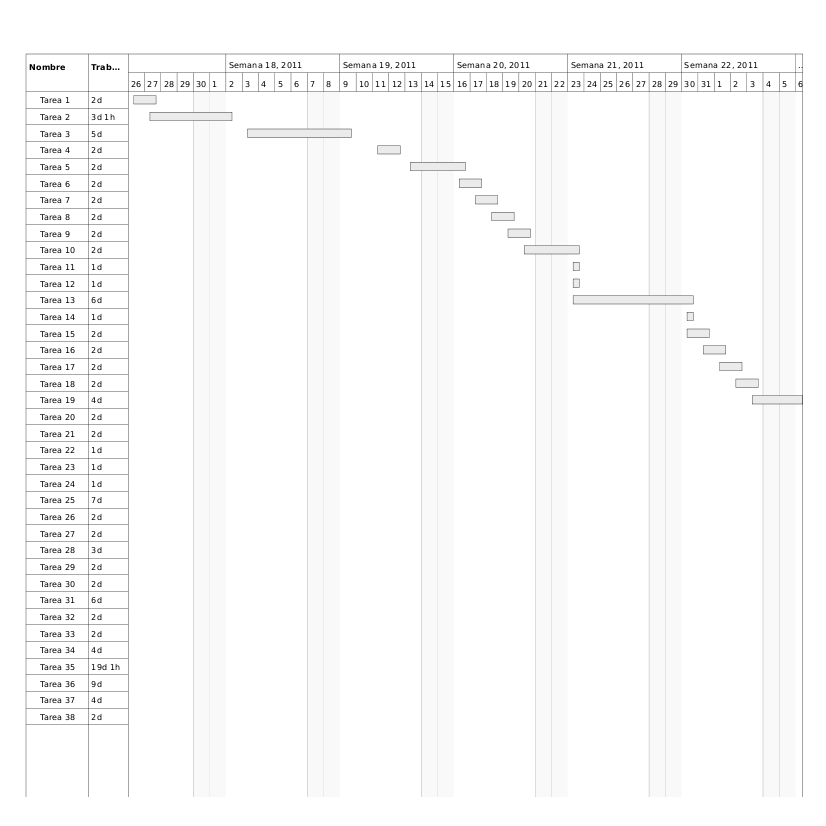
\includegraphics[width=18.5cm]{diagrama_gantt_uno.png}}
\caption{Planificación Temporal del proyecto - Desde el 26 de Abril}
\end{figure}

\pagebreak
\begin{figure}[H]
\hspace*{-.5in}{
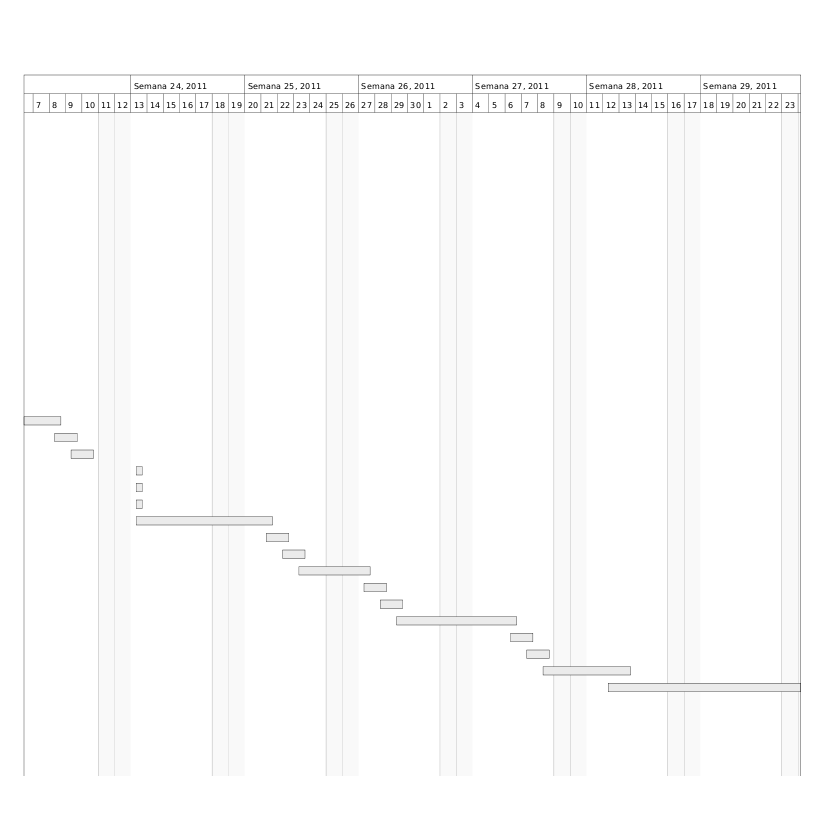
\includegraphics[width=18.5cm]{diagrama_gantt_dos.png}}
\caption{Planificación Temporal del proyecto - Desde el 6 de Junio}
\end{figure}

